\chapter{Architecture Implementation}
In the following chapter we present the implementation of the individual decompositions as described in figure \ref{fig:comp}.

It should be noted, that although Astah claimed \gls{rte} support for C++, it was found to be unreliable, due to poor support of the C++ namespace feature.
The application was thus developed using a conventional model-driven design approach.

\section{Main Application}
The core functionality of the program was established in section \ref{sec:archplug} to be
\begin{itemize}
	\item Configuration storage
	\item Plugin management
	\item Curve rendering to screen
	\item \gls{cli} parsing
\end{itemize}

These components lead to a further decomposition as per figure \ref{fig:main}.

\begin{figure}[htb]
	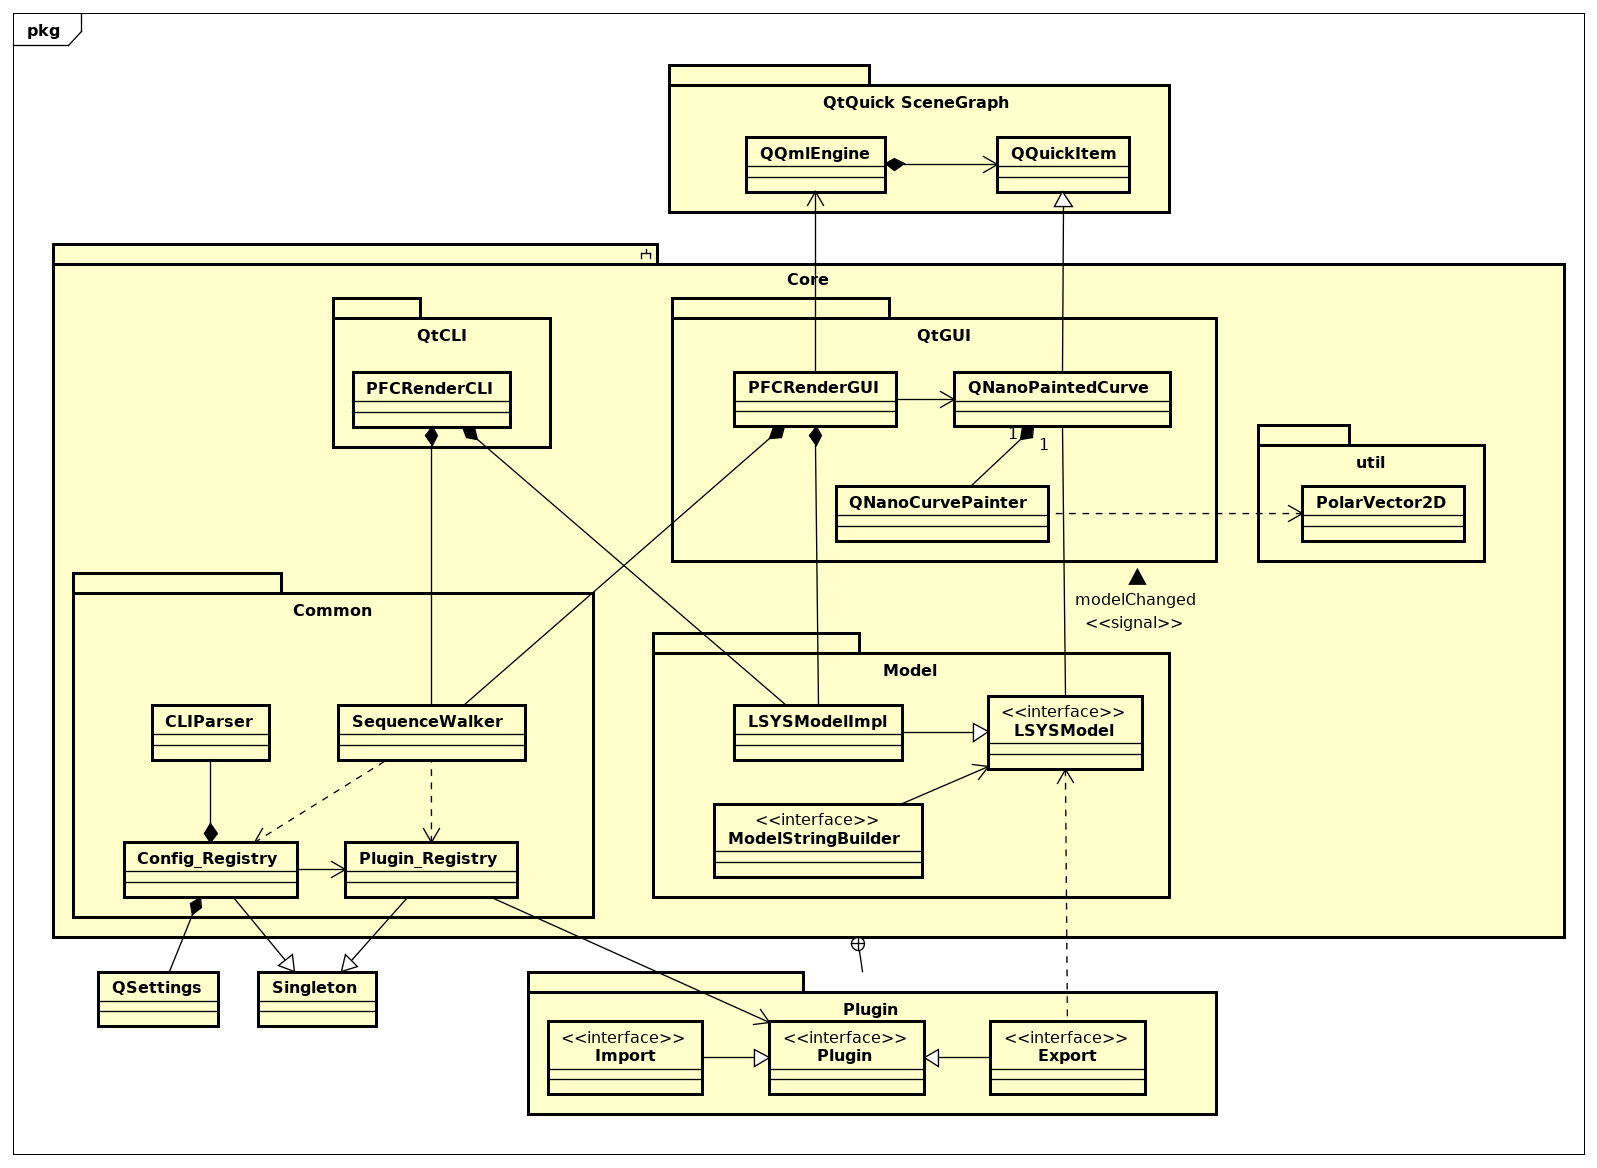
\includegraphics[width=\textwidth]{MainAppClassDiagram}
	\caption{Class Structure of Core Application}
	\label{fig:main}
\end{figure} 

\paragraph{Initialization and Operation}
The main entry point into the application is not shown here in the class diagram, but it involves creating a Qt specific QGuiApplication object and a PFCRenderGUI or PFCRenderCLI object.

In case of \gls{gui} operation, a QQmlEngine is instantiated to handle the declarative \gls{gui} part and the Qt event loop is executed through the QGuiApplication. A SequenceWalker then handles requested operations, upon completion of which the \gls{gui} starts handling all further interaction asynchronously through a Qt specific messaging system called Signals and Slots, which utilizes said event loop.

In batch mode, the PFCRenderCLI simply calls the SequenceWalker class, which handles all requested operations and then exits.

\paragraph{Configuration}
Config\_Registry is the central store of configuration information as outlined in \ref{sec:archconf} and - upon creation of its instance (which happens the first time some class wants to access configuration data) resolves the sequence of reading settings from file, creating the Plugin\_Registry to query for options, and parsing the CLI. It is also available to the QML part of the application as an exported QML type, allowing GUI screens written in QML to access config data.

\paragraph{Plugins} Since Plugins need to be loaded to query for config information anyway, it makes sense to hold references to them active, so they do not have to be loaded a second time once accessed for execution. Plugin\_Registry is a second Singleton tasked with resolving all available plugins and holds this reference associated with plugin name for easy lookup.

\paragraph{Model Creation} The model is created once on startup of the application via the PFCRender* objects. Once the sequence walker executes an import plugin, it will be given a ModelStringBuilder object to execute. Upon completion, it pushes an owning \cmd{std::unique\_ptr<>} to that string to the model to avoid potentially costly string copying.

Benefit of a returned builder object instead of direct plugin invocation is deferred/delegated execution, as it becomes simple for the sequence walker to hand the builder over to a thread. This helps with keeping the \gls{gui} responsive while computation occurs in the background. This feature is planned for a subsequent release, as it was not a direct requirement.

\paragraph{GUI Creation} The \gls{gui} is loaded from \gls{qml} files on startup, the QNanoPaintedCurve displaying an empty rendering. It is connected to the modelChanged signal and - on notification of a change - copies the model string to its renderer - QPainterParse. It then notifies the QSGSceneGraph it wants to be redrawn, which invokes the QPainterParse::paint() function when re-rendering, which parses the string into actual geometry. On completed rendering, the QNanoPaintedCurve notifies the \gls{qml} part of the \gls{gui} if its \gls{bounding box} has changed, in order to scale the result to the available window size.

\paragraph{Export} The sequence walker extracts the model string and hands it over to the plugin, which is then free to do its job, while getting configuration from the config\_registry.

\subsection{Challenges Faced in Rendering the Model Curve}
Had performance not been a direct requirement, the QPainter API would have been sufficiently sophisticated to enable curve drawing. Since QPainter is too slow - as found in section \ref{sec:qtrender} - an alternative approach is necessary.

The first studied alternative was direct scene graph node manipulation, which turned out to be too inflexible to satisfy all requirements.

An alternative was ultimately adopted with of using QNanoPainter.

We will now discuss challenges faced with both rendering methods.

\subsubsection{Direct node instertion into the scene graph}
While QQuickPaintedItem allows us to use the QPainter API to generate the model for viewing, which is great, since it is also used by the SVG and PDF exporters, it is also painfully slow, as running callgrind on two parallel implementations shows.
do\_paint, which renders using QPainter API is a factor of 10 slower than manual creation of the OpenGL Vertex/Colordata

IMAGE : Callgrind cost

For this reason, a parallel implementation of both approaches was selected, with the GUI using rendering directly, and Painter based exporters using the QPainter API.

While this means that the GUI viewmodel can not be reused and the curve has to be rebuilt using qpainter on export, the GUI becomes responsive more quickly / scales to more iterates. As far as UX goes, the user can wait for file export, but not for an interactive GUI.
Especially since export is threadable/backgroundable.

rcs bezier
\subsubsection{Calculating the bounding box}
Drawing the geometry from the string is an iterative process in nature. The the final size and position of the curve is not known until after the full curve is constructed.

It is necessary to relocate and rescale the drawing in order to fit it on the output device used  (screen, printer page size). There are two approaches to this:
\begin{itemize}
	\item Go through the string once, just to gather min and max coordinates to create the bounding box. Apply coordinate transformation to the drawing tool and reparse the string.
	\item Pick up the bounding box while drawing the geometry. Apply the necessary transformation afterwards.
\end{itemize}
Regarding the performance impact of iterating through a potentially very long string a second time, the latter is obviously preferable. The iterative drawing frameworks QPainter and QNanoPainter do not provide any facility to apply scaling after drawing has been done, as they place actual rendering calls using the current rendering engine (OpenGL or OpenGLES).

For the \gls{gui}, which required to load fast, a solution for this problem was found. As QNanoPainter does not issue drawing calls directly upon execution, but queues them up to be drawn when the scene graph reaches the current node, it is possible to apply the necessary transformations in a parent node, which - as per the logic of the scene graph - applies to all child nodes.

As no such deferred drawing is possible when using QPainter to print to PDF, the bounding box is precalculated and applied to the calls directly. Since file export is not a time critical operation, this reparsing is considered tolerable.

Using the translate property, which - under the hood - prepends the actual scenegraph node with a QSGTransformNode, the rendering can be done without concern for target coordinates and moved to fit the window after drawing.

\subsection{QNanoPainter Stringcopy}

Copying the model string cna nnot be avoided!


It turned out that QNanoPainter forces the scene graph managed by Qt to call QNanoQuickItemPainter::paint() function, which in our case is used to create the texture from the model string, on every frame, leading to a unusable \gls{gui} on complex models.

\todo{maybe elaborate on the scene graph in architecture def}
When the scene graph collects data for rendering, it reuses cached data if it has not changed for efficiency. To indicate changes that need redrawing, dirty bits are set on that node, which specify in which way a node's data has changed. In the case of QNanoPainter 

\begin{lstlisting}[language=c++,caption=QNanoQuickItem as of commit de45f31e]
QSGNode *QNanoQuickItem::updatePaintNode(QSGNode *node, QQuickItem::UpdatePaintNodeData *nodeData)
{
    Q_UNUSED(nodeData)
    QNanoQuickItemPainter *n = static_cast<QNanoQuickItemPainter *>(node);
    if (!n) {
        n = createItemPainter();
    }
    n->synchronizePainter(this);
    n->markDirty(QSGNode::DirtyMaterial);
    return n;
}
\end{lstlisting}
This code calls \code{markDirty()} on every execution, forcing the scene graph to call the QNanoCurvePainter::paint() function to redraw the geometry.

This behavior is probably intended, as QNanoPainter can also draw on QQuickFramebufferObject as a backend, which does not have the notion of dirtyness, so this was likely inplemented for consistency in user code.

We resolved this problem by forking QNanoPainter, removing this call from \code{updatePaintNode()} and calling it in the QNanoCurvePainter::synchronize method instead, which is called by synchronizePainter() in the above snippet, but is a class implemented by the user, thus exposing control over whether to redraw or not to the user. A pull request to the official repository will be submitted shortly.

\subsection{Angle calculation}
\begin{quote}
Sometimes "pi = 3.14" is (a) infinitely faster than the "correct" answer and (b) the difference between the "correct" and the "wrong" answer is meaningless. And this is why I get upset when somebody dismisses performance issues based on "correctness". The thing is, some specious value of "correctness" is often irrelevant because it doesn't matter. While performance almost always matters. And I absolutely detest the fact that people so often dismiss performance concerns so readily.

- Git mailing list, Fri, 8 Aug 2008
\end{quote}

\subsubsection{Encapsulation of Functionality (OOP) vs. Method Call overhead}
A lot of the OOP functionalites C++ offers, come at a performance cost.
While some of those classically named ones like stl containers are almost equivalent to plain C data, there are still very costly abstractions present in C++ wwhich can slow down a program significantly.
The gaming world programs C++ without exceptions for this exact reason (TODO: Reference), while those don't come into play here, method call overhead does.

\subsubsection{Polymorphism and Performance}
Polymorphic classes are a key abstraction of C++ and are distinct from simple inheritance by the presence of the virtual keyword on at least some of their members.

This keyword enables a derived class, referred to through a pointer to the base class to execute its own implementation (a so called override) of the virtual member instead of the one (possibly, but not necessarily) implemented by the base class.

While this mechanism is fundamental to enabling C++ to provide the so called interface abstraction (TODO:Define), it comes with a performance cost.

Calls to a virtual function are not made by directly accessing the address of the callee, but access the so-called vtable instead. which is tasked with resolving the address of the member function.

This introduces several additional cycles (TODO: Measure how many or find in literature), which can become a significant bottleneck for performance, when the virtual function is called often, e.g. in our case, when parsing a character of the model string.



\section{Plugins}
\subsubsection{Inheritance in Qt}
Implementing interfaces that are supposed to be used with Qt's meta object system is a slightly awkward procedure, as Qt's macros used to notify the moc about interface definitions and implementations are not namespace aware. 

This limitation pertains to interfaces exposing functionality from the Qt MetaObject system like signals/slots.

\begin{figure}[htb]
	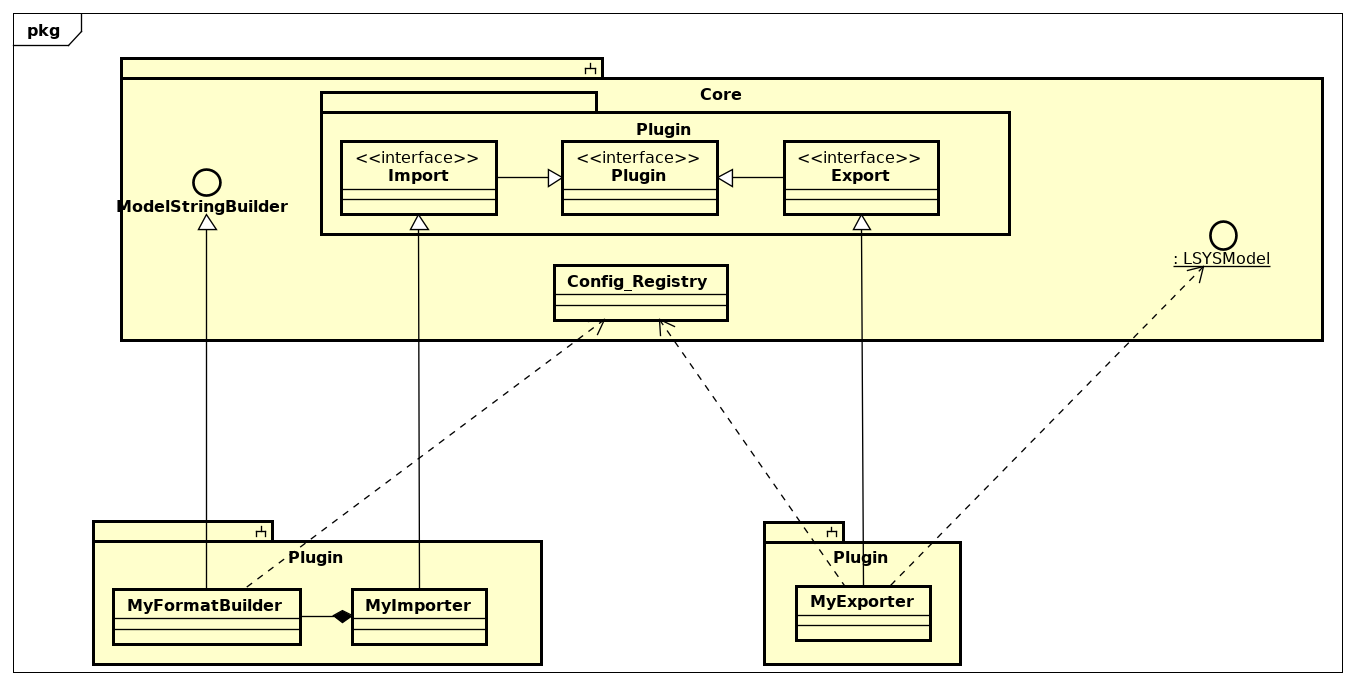
\includegraphics[width=\textwidth]{PluginInterface}
	\caption{Plugin Interface}
	\label{fig:plugint}
\end{figure}

\section{\gls{lsys} Input}
\label{sec:lsys}
\section{SVG Output}
\label{sec:svg}

\section{PDF Output}
\label{sec:pdf}


\subsection{Build System}
As stated previously, Travis CI
Setting up the \gls{ci} environment is a pain, mainly caused by Travis using a 6 year old Linux distribution by default, where the standard version of gcc is 4.8, which does not even support C++11.

\subsection{CI}
Since switching to the NanoVG based QNanoPainter, Appveyor windows builds are failing with unresolved externals, all of which are gl*() OpenGL functions.


On Ubuntu 14.04, no GLES3 installation is present, this could be worked around by forcing QNanoPainter to use GLESv2.

This was non-trivial to set up though, as Qt is by default not linked to a specific graphics backend - i.e. linking has to be done manually for QNanopainter to work

Thankfully developers encountered the same problem and solved it for the qmake buildsystem, fixing it amounted to adapting their solution to CMAke.

\section{Automated Unit Testing and Coverage Reporting}
A main benefit of using Github - as already stated, is the third party tool integration offered.

Regarding unit testing, this results in the possibility to not only automatically run tests on each build of Travis CI, but also visualize the \gls{coverage} of the tests executed using \url{codecov.io}, which hooks into Travis completed builds that generated code output with coverage information and generates a graphical report on which lines of code were actually executed during testing.

They turned out to eat up about as much productivity in maintenance as they freed

Travis CI runs on Ubuntu 12.04LTS which reached End-of-Life in 2017. Ubuntu 14.04LTS support is still experimental, but even with the updated OS, the available tools are heavily outdated.

Huge benefit to maintainability, clear insight on testing, fast feedback whether changes work.

Standard gcc is a v4 with no support for C++11
Manually updating tools had ramifications as gcov was now ouptutting coverage data from gcov-5, lcov was using the old gcov-4 leading to no coverage being reported. Manually setting the gcov tool path resolved this issue, which - along with the time spent identifying the problem - was a significant time drain.

Still, the great benefit of this tool is that once it has been set up, it "just works" - running alongside the projects dev flow unintrusively and gives good insight into areas of improvement.
\todo{lolwut}

